\documentclass[a4paper,12pt]{article}
\usepackage{a4wide}
\usepackage{tikz}
\usetikzlibrary{calc}
\usepackage{hyperref}
\usepackage{color}
\usepackage{pdflscape}
\usepackage{bytefield}

\usepackage[ngerman]{babel}

\newlength{\maxheight}
\setlength{\maxheight}{\heightof{W}}
\newcommand{\baselinealign}[1]{ %
	\centering
	\raisebox{0pt}[\maxheight][0pt]{ #1}%
}

\newcommand\Tstrut{\rule{0pt}{2.6ex}}       % "top" strut

\definecolor{grau}{gray}{.5}

\begin{document}
\pagestyle{empty}
\setlength{\parindent}{0em}
\section*{Single Cycle Control Unit}

Ihre Aufgabe ist es, das Verhalten einer Entity  namens "`SC\_CU"' zu programmieren. Die Entity ist in der angeh\"angten Datei "`SC\_CU.vhdl"' deklariert und hat folgende Eigenschaften:
\begin{itemize}
\item Eingang:  Opcode vom Typ std\_logic\_vector mit einer L\"ange von 6
\item Eingang:  Funct vom Typ std\_logic\_vector mit einer L\"ange von 6
\item Eingang:  Zero vom Typ std\_logic
\item Ausgang: ALUControl vom Typ std\_logic\_vector mit einer L\"ange von 3
\item Ausgang: Steuersignale RegDst, Branch, Jump, MemRead, MemtoReg, MemWrite, ALUSrc and RegWrite alle vom Typ std\_logic
\end{itemize}

\begin{center}
\begin{tikzpicture}
\draw node [draw,rectangle, minimum height=55mm, minimum width=35mm,rounded corners=2mm,thick](entity){};

\draw[->] ($ (entity.west)+(-10mm,10mm)$) -- ($ (entity.west) + (0mm,10mm)$);
\draw node at ($ (entity.west)-(18mm,-10mm)$){Opcode};

\draw[->] ($ (entity.west)-(10mm,0mm)$) -- ($ (entity.west) - (0mm,0mm)$);
\draw node at ($ (entity.west)-(16mm,0mm)$){Funct};

\draw[->] ($ (entity.west)-(10mm,10mm)$) -- ($ (entity.west) - (0mm,10mm)$);
\draw node at ($ (entity.west)-(15mm,10mm)$){Zero};


\draw[->] ($ (entity.east) + (0mm,24mm)$) -- ($ (entity.east) + (10mm,24mm)$);
\draw node at ($ (entity.east) + (18mm,24mm)$){RegDst};

\draw[->] ($ (entity.east) + (0mm,18mm)$) -- ($ (entity.east) + (10mm,18mm)$);
\draw node at ($ (entity.east) + (18mm,18mm)$){Branch};

\draw[->] ($ (entity.east) + (0mm,12mm)$) -- ($ (entity.east) + (10mm,12mm)$);
\draw node at ($ (entity.east) + (17mm,12mm)$){Jump};

\draw[->] ($ (entity.east) + (0mm,6mm)$) -- ($ (entity.east) + (10mm,6mm)$);
\draw node at ($ (entity.east) + (21mm,6mm)$){MemRead};

\draw[->] ($ (entity.east) + (0mm,0mm)$) -- ($ (entity.east) + (10mm,0mm)$);
\draw node at ($ (entity.east) + (21.5mm,0mm)$){MemtoReg};

\draw[->] ($ (entity.east) + (0mm,-6mm)$) -- ($ (entity.east) + (10mm,-6mm)$);
\draw node at ($ (entity.east) + (21.3mm,-6mm)$){MemWrite};

\draw[->] ($ (entity.east) + (0mm,-12mm)$) -- ($ (entity.east) + (10mm,-12mm)$);
\draw node at ($ (entity.east) + (22.5mm,-12mm)$){ALUControl};

\draw[->] ($ (entity.east) + (0mm,-18mm)$) -- ($ (entity.east) + (10mm,-18mm)$);
\draw node at ($ (entity.east) + (18.5mm,-18mm)$){ALUSrc};

\draw[->] ($ (entity.east) + (0mm,-24mm)$) -- ($ (entity.east) + (10mm,-24mm)$);
\draw node at ($ (entity.east) + (20mm,-24mm)$){RegWrite};

\draw node at ($ (entity) - (0,0mm)$){SC\_CU};

\end{tikzpicture}
\end{center}

Ver\"andern sie die Datei "`SC\_CU.vhdl"' nicht!
\\

Sie m\"ussen folgende verschiedene Instruktions-Typen implementieren:
{{SELECTED_INSTRUCTIONS_TYPE}}

Die Entity soll den Single Cycle Prozessor, welcher in Abbildung~1 dargestellt ist, so steuern, dass folgende Instruktionen ausgef\"uhrt werden k\"onnen:

\begin{table}[h!]
\centering
    \begin{tabular}{|c|c|c|c|c|} \hline \Tstrut
		instruction & opcode  & funct	& zero & type   \\ \hline \Tstrut
		{{SELECTED_INSTRUCTIONS}}
    \hline
    \end{tabular}
\end{table}

{{SELECTED_INSTRUCTIONS_TEXT}} \\

\begin{table}[h!]
\centering
    \begin{tabular}{|c|c|} \hline \Tstrut
		ALUControl & Befehl   \\ \hline \Tstrut
		{{SELECTED_ALUCONTROLS}}
    \hline
    \end{tabular}
    \caption{ALUControls}
    \label{tab:ALUControls}
\end{table}


Um ein besseres Verst\"andnis f\"ur die Steuersignale zu erhalten, sei hier eine Beschreibung aller Signale gegeben. Verwenden Sie Abbildung~1 um zu verstehen, wie die Steuersignale die Datenpfade steuern.
\begin{itemize}

	\item{RegDst: Bestimmt, ob die Position des zu beschreibenden Registers "`Write Register"' entweder von den Bits 20 -- 16 oder 15 -- 11 der Instruktion definiert wird. In anderen Worten entscheidet dieses Steuersignal, ob das zu beschreibende Register durch rt oder rd festgelegt wird.}

	\item{Branch: Hat einen Effekt auf die Quelle f\"ur den n\"achsten Wert des Befehlsz\"ahlers (PC). Wenn die Branch Bedingung erf\"ullt ist, ist der Wert '1'. Ist die aktuelle Instruktion keine Branch Instruktion, so ist der Wert immer '0'.}

	\item{Jump: Hat einen Einfluss auf die Quelle f\"ur den n\"achsten Wert des Befehlsz\"ahlers (PC). Ist die aktuelle Instruktion keine Jump Instruktion, so ist der Wert immer '0'.}

	\item{MemRead: Wenn das MemRead Signal auf '1' gesetzt ist, dann gibt der Datenspeicher "`Data memory"' jene Daten aus, welche durch den Adresseingang "`Read address"' bestimmt werden.}

	\item{MemtoReg: Bestimmt, ob die in das Register zu schreibenden Daten "`Write data"' entweder vom Ausgang des Datenspeichers "`Data memory"' oder dem ALU Ausgang "`Result"' kommen.}

	\item{MemWrite: Wenn dieses Signal auf '1' gesetzt ist, dann schreibt der Datenspeicher "`Data memory"' seine Eingangsdaten ("`Write data"') an die Zieladresse "`Write address"'.}

	\item{ALUControl: W\"ahlt jene ALU Operation aus, welche die ALU auf ihre zwei Eingangswerte anwendet. Die Steuersignale f\"ur die verf\"ugbaren Operationen sind in Tabelle~1 gelistet.}

	\item{ALUSrc: Bestimmt, ob die ALU einen Wert entweder von dem Ausgang "`Read data 2"' des Registers oder von dem vorzeichenerweiterten Wert IMM der Instruktion erh\"alt.}

	\item{RegWrite: Wenn das RegWrite Signal auf '1' gesetzt ist, dann schreibt das Register die Eigangsdaten "`Write data"' in das durch "`Write register"' adressierte Register.\\}

\end{itemize}

\"Uberlegen Sie sich, welche Aktion jeder Teil des Prozessors f\"ur die Funktion der jeweiligen Instruktionen erf\"ullen muss und setzen Sie die Steuersignale entsprechend. Programmieren Sie dieses Verhalten in der angeh\"angten Datei "`SC\_CU\_beh.vhdl"'.\\

Um Ihre L\"osung abzugeben, senden Sie ein E-Mail mit dem Betreff "`Result Task {{ TASKNR }}"' und Ihrer Datei "``SC\_CU\_beh.vhdl"'  an {{ SUBMISSIONEMAIL }}.

\vspace{0.5cm}

Viel Erfolg und m\"oge die Macht mit Ihnen sein.

\begin{landscape}
\begin{figure}[!h]
\vspace{-0.5cm}
\hspace{-1.8cm}
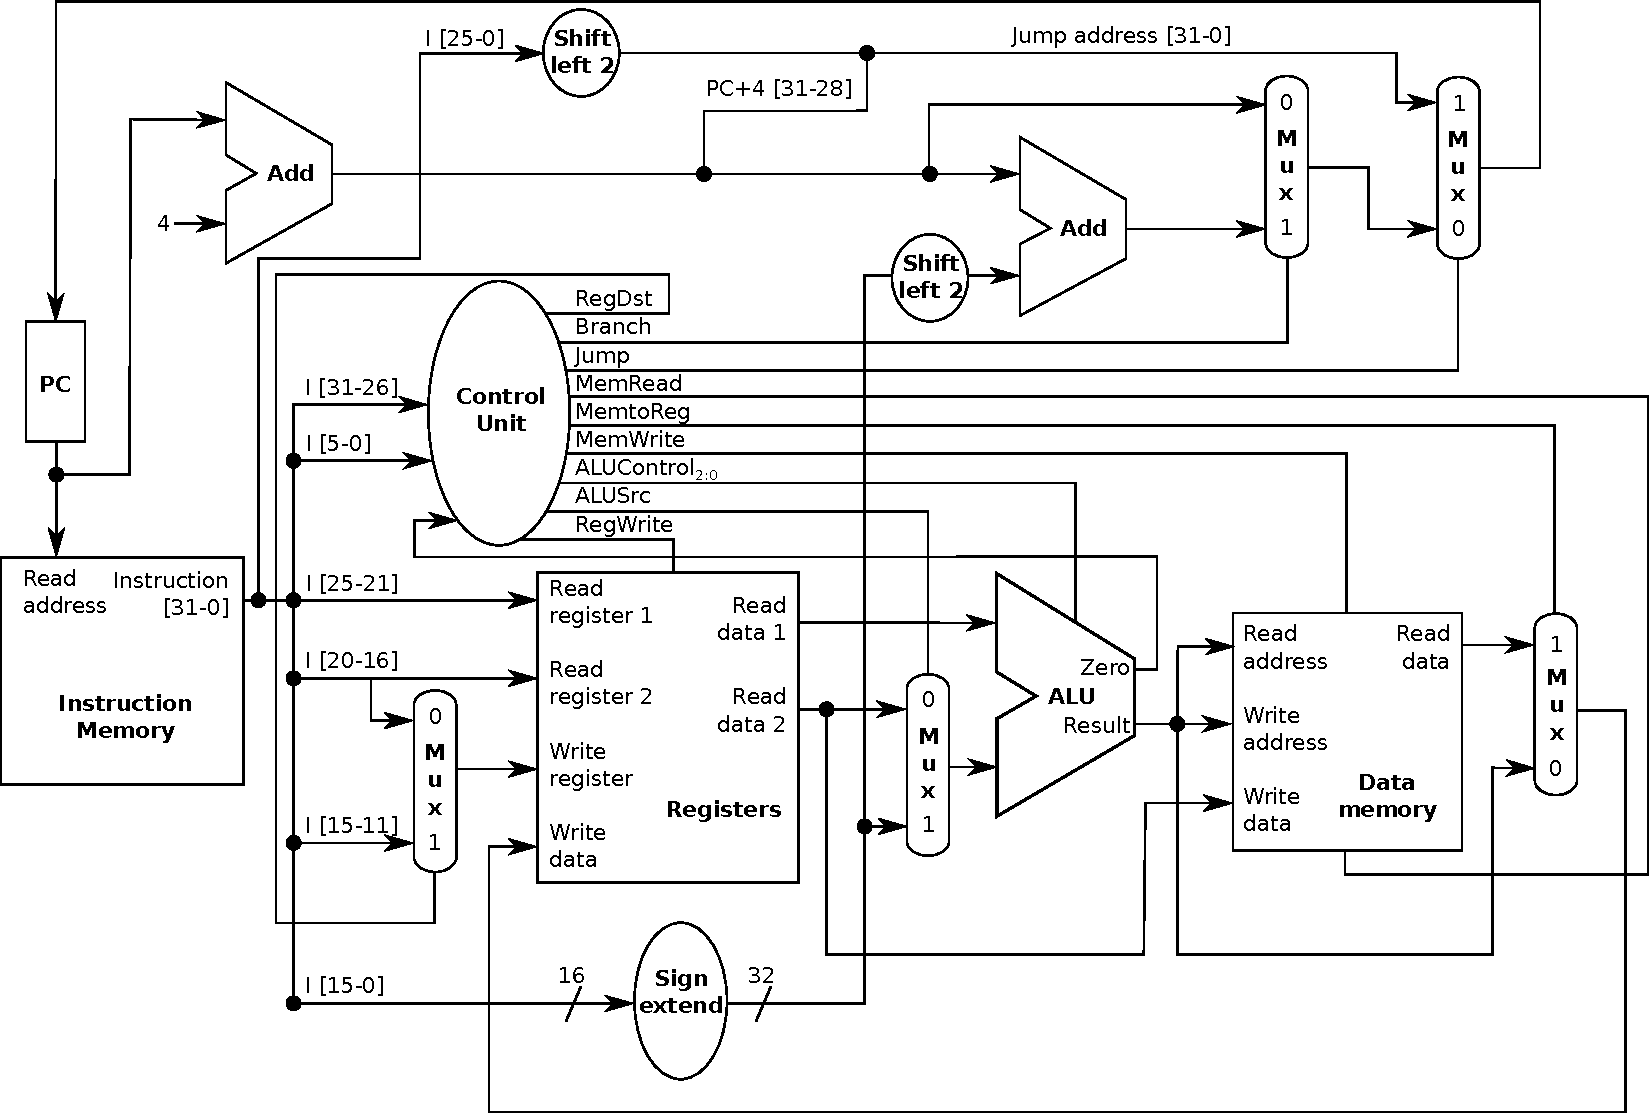
\includegraphics[width=25.5cm]{Single_Cycle_Processor_V_3_0}
\caption{Single Cycle Prozessor}
\label{fig:SingleCycleProcessor}
\end{figure}
\end{landscape}


\end{document}
